\documentclass[12pt,a4paper]{article}
\usepackage[utf8]{inputenc}
\usepackage[T2A]{fontenc}
\usepackage[russian]{babel}
\usepackage{amsmath, amssymb, amsthm}
\usepackage{geometry}
\geometry{a4paper, top=2.0cm, bottom=2.0cm, left=3.0cm, right=1.5cm}
\usepackage{booktabs}
\usepackage{graphicx}
\usepackage{hyperref}

\hypersetup{
	colorlinks=true,
	linkcolor=black,
	filecolor=black,      
	urlcolor=blue,
	citecolor=black,
}


\newtheorem{theorem}{Теорема}
\newtheorem{lemma}{Лемма}
\newtheorem{definition}{Определение}
\newtheorem{proposition}{Утверждение}
\newtheorem{corollary}{Следствие}

\begin{document}
	

	\begin{titlepage}
		\begin{center}
			{\large Санкт-Петербургский государственный университет}\\[0.5cm]
			{\large Направление: Прикладная математика и информатика}\\[4.5cm]
			
			{\Large \bfseries ОТЧЕТ}\\[0.3cm]
			{\large по учебной практике (научно-исследовательской работе)}\\[0.3cm]
			{\large (семестр 2)}\\[2.5cm]
			
			{\Large \bfseries Экстраградиентные и оптимистичные методы в
				обучении GAN:
				вариационные неравенства, монотонность и устойчивость
				состязательного генеративного обучения}\\[4.5cm]
		\end{center}
		
		\begin{flushright}
			\begin{tabular}{l}
				\textbf{Выполнил:}\\
				студент группы 25.Б21-мм\\
				Самвелян Артур Хачатурович\\[0.8cm]
				\textbf{Научный руководитель:}\\
				Мокаев Тимур Назирович
			\end{tabular}
		\end{flushright}
		
		\vfill
		
		\begin{center}
			Санкт-Петербург\\
			2026
		\end{center}
	\end{titlepage}
	

	\newpage
	\tableofcontents
	\newpage
	

	
	\section{Введение}
	
	Обучение генеративно-состязательных сетей (GAN) представляет собой динамическую игру двух участников - генератора и дискриминатора, где вместо привычной минимизации одной функции потерь ставится задача поиска седловой точки или равновесия Нэша в минимаксной задаче. В рамках исследований предыдущего семестра был подробно изучен локальный линейный анализ этой состязательной динамики: исследовались свойства матрицы Якоби, её разложение на симметричную и кососимметричную части, а также влияние различных методов стабилизации, таких как штрафы на градиент (R1-регуляризация), добавление шума на входе дискриминатора (Instance noise) и двухмасштабные схемы шагов (TTUR). Было показано, что в игровой динамике антисимметричная часть Якобиана вызывает циклическое вращение траекторий параметров параметров, в то время как симметричная часть отвечает за диссипацию и локальную устойчивость.
	
	Однако локальный линейный анализ в окрестности стационарной точки не способен в полной мере описать глобальное поведение алгоритмов и их сходимость вне малой окрестности равновесия. Естественным развитием исследования является переход к более общей, строгой  математической постановке - языку вариационных неравенств и теории монотонных операторов. Настоящая работа посвящена исследованию связи между локальным спектральным анализом Якобиана и глобальными понятиями монотонности, псевдомонотонности. 
	\section{Терминология, цель работы, постановка задачи}

	Во избежание смешения различных соглашений, при оформлении работы используется следующий единый терминологический стиль:
	\begin{itemize}
		\item \textbf{Генеративно-состязательная сеть (GAN)} - архитектура машинного обучения, моделирующая распределение данных через минимаксную игру генератора и дискриминатора.
		\item \textbf{Экстраградиентный метод} - двухшаговый алгоритм оптимизации, использующий промежуточное (предикторное) вычисление градиента для стабилизации игровой динамики.
		\item \textbf{Оптимистичный градиентный метод} - метод обучения, использующий экстраполяцию шага за счет истории градиентов с предыдущей итерации.
		\item \textbf{Двухмасштабное правило обновления (TTUR)} - схема выбора гиперпараметров, задающая разные (асимметричные) скорости обучения для участников игры.
		\item \textbf{Вариационное неравенство} - общая математическая постановка, позволяющая находить равновесные состояния систем через поиск нуля связанного операторного поля.
		\item \textbf{Монотонный оператор} - свойство векторного поля, гарантирующее отсутствие локальных максимумов/минимумов и определяющее глобальную сходимость алгоритмов.
	\end{itemize}
	
	\subsection{Цель работы}
	Основная цель работы заключается в переходе от локального линейного анализа к более общей и концептуально цельной постановке. Главная идея состоит в том, чтобы рассматривать обучение GAN как задачу поиска решения вариационного неравенства или седловой задачи, а также проследить связь между локальным спектральным анализом якобиана и более глобальными понятиями монотонности, псевдомонотонности и устойчивости.
	
	\subsection{Постановка задачи}
	Для достижения поставленной цели необходимо выполнить следующие задачи:
	\begin{enumerate}
		\item Сформулировать классическую постановку GAN как минимаксной задачи.
		\item Ввести связанное векторное поле игры и объяснить, как из него возникает постановка вариационного неравенства.
		\item Разобрать смысл понятий монотонности, сильной монотонности, псевдомонотонности и их связь с устойчивостью обучения.
		\item Объяснить, почему для игровой динамики антисимметричная часть якобиана вызывает вращение и циклы, а симметричная часть отвечает за диссипацию и локальную устойчивость.
		\item Выполнить теоретическую часть:  вывести переход от минимаксной задачи GAN к операторной постановке и рассмотреть билинейную игру как модельный пример.
		\item Сопоставить экстраградиентный и оптимистичный подходы: объяснить их математическое сходство и различие, а также сформулировать, какие именно механизмы подавляют вращение в игре.
		\item Выполнить практическую часть: реализовать вычислительные эксперименты в Python/PyTorch на примере toy-GAN на двумерных данных. Провести сравнение методов vanilla gradient descent-ascent, extragradient и optimistic gradient.
		\item Провести абляционный анализ: изучить влияние шага обучения на устойчивость, а также отдельно проверить, как меняются результаты при добавлении слабой регуляризации или шума.
		\item Подготовить воспроизводимый репозиторий с исходным кодом, инструкцией по запуску, фиксированными seed и скриптами построения графиков и таблиц.
	\end{enumerate}
	
	\section{Основная часть}
	
	\subsection{Краткий конспект}
	\subsubsection{Векторное поле игры и вариационные неравенства}
	Классическая задача обучения генеративно-состязательных сетей формулируется как минимаксная оптимизация:
	\begin{equation}
		\min_{\theta_G} \max_{\theta_D} V(\theta_G, \theta_D),
	\end{equation}
	где $V$ - целевая функция, $\theta_G$ и $\theta_D$ - параметры генератора и дискриминатора соответственно. 
	
	Для анализа динамики обучения градиентными методами удобно объединить параметры в единый вектор $\theta = (\theta_G, \theta_D)$ и ввести связанное векторное поле игры:
	\begin{equation}
		F(\theta) = \begin{pmatrix}
			\nabla_{\theta_G} V(\theta_G, \theta_D) \\
			-\nabla_{\theta_D} V(\theta_G, \theta_D)
		\end{pmatrix}.
	\end{equation}
	В непрерывном времени стандартный градиентный спуск-восход (GDA) описывается дифференциальным уравнением $\dot{\theta} = -F(\theta)$. Поиск локального равновесия Нэша без ограничений сводится к нахождению стационарной точки $\theta^*$, в которой $F(\theta^*) = 0$. 
	
	В более общем случае, когда параметры принадлежат некоторому выпуклому компактному множеству $\Theta$, задача эквивалентна решению \textbf{вариационного неравенства}. Требуется найти такую точку $\theta^* \in \Theta$, что для всех $\theta \in \Theta$ выполняется:
	\begin{equation}
		\langle F(\theta^*), \theta - \theta^* \rangle \ge 0.
	\end{equation}
	
	
	\subsubsection{Монотонность и устойчивость обучения}
	В теории вариационных неравенств ключевую роль играют свойства оператора $F$, которые определяют характер сходимости алгоритмов.
	\begin{itemize}
		\item \textbf{Монотонность (Monotonicity):} Оператор $F$ называется монотонным, если для любых $\theta, \theta'$ выполняется $\langle F(\theta) - F(\theta'), \theta - \theta' \rangle \ge 0$. Геометрически это означает, что векторное поле направлено «внутрь» к равновесию. В строго монотонных полях градиентная динамика не расходится, однако может приводить к бесконечным осцилляциям вокруг стационарной точки.
		\item \textbf{Сильная монотонность (Strong Monotonicity):} Выполняется условие $\langle F(\theta) - F(\theta'), \theta - \theta' \rangle \ge \mu \|\theta - \theta'\|^2$ для некоторого $\mu > 0$. Это наиболее жесткое условие, гарантирующее экспоненциально быструю сходимость градиентных методов к единственному равновесию.
		\item \textbf{Псевдомонотонность (Pseudomonotonicity):} Ослабленное условие, при котором из $\langle F(\theta'), \theta - \theta' \rangle \ge 0$ следует $\langle F(\theta), \theta - \theta' \rangle \ge 0$. Это свойство часто является наиболее реалистичным предположением для глубоких нейронных сетей, при котором методы с экстраполяцией все еще могут гарантировать достижение стационарной точки.
	\end{itemize}
	
	\subsubsection{Спектральный анализ Якобиана и игровая динамика}
	Локальное поведение системы в окрестности равновесия определяется матрицей Якоби $J(\theta) = \nabla F(\theta)$. Матрицу $J$ можно однозначно разложить на симметричную и антисимметричную (кососимметрическую) части:
	\begin{equation}
		J = S + A, \quad \text{где } S = \frac{J + J^\top}{2}, \quad A = \frac{J - J^\top}{2}.
	\end{equation}
	Каждая из этих частей играет  разную роль в динамике обучения:
	\begin{itemize}
		\item \textbf{Антисимметричная часть ($A$):} Отражает состязательную (игровую) природу GAN. Все ненулевые собственные значения матрицы $A$ являются чисто мнимыми. Динамика, порождаемая этой частью, строго ортогональна градиенту расстояния до оптимума, что вызывает непрерывное вращение траекторий и циклы.
		\item \textbf{Симметричная часть ($S$):} Отражает  оптимизационную природу. Если $S$ положительно определена (собственные значения вещественны и положительны), она действует как демпфер, обеспечивая  притягивание траектории к локальному равновесию.
	\end{itemize}
	В стандартном методе градиентного спуска-восхода антисимметричная часть часто доминирует, что приводит к нестабильности. Для компенсации вращательного момента необходимо использовать методы, неявно модифицирующие Якобиан системы. Например, алгоритмы оптимистичного градиентного спуска и экстраградиентные методы используют информацию из прошлых шагов для аппроксимации будущего состояния векторного поля, что математически эквивалентно добавлению положительно определенной  компоненты к эффективной матрице итерации, тем самым обеспечивая локальную устойчивость.
	

	



	\subsection{Теоретическая часть}
	\subsubsection{Переход от минимаксной задачи к операторной постановке}
	Классическая задача обучения генеративно-состязательных сетей формулируется как минимаксная игра двух лиц с нулевой суммой:
	\begin{equation}
		\min_{x \in \mathcal{X}} \max_{y \in \mathcal{Y}} V(x, y),
	\end{equation}
	где $x$ --- параметры генератора, $y$ --- параметры дискриминатора. 
	
	Необходимым условием первого порядка для внутреннего равновесия Нэша $(x^*, y^*)$ является равенство нулю градиентов по обоим аргументам: $\nabla_x V(x^*, y^*) = 0$ и $\nabla_y V(x^*, y^*) = 0$. 
	
	Объединим параметры в единый вектор $z = (x, y) \in \mathcal{Z} = \mathcal{X} \times \mathcal{Y}$ и определим связанное векторное поле игры (оператор) $F(z)$ следующим образом:
	\begin{equation}
		F(z) = \begin{pmatrix}
			\nabla_x V(x, y) \\
			-\nabla_y V(x, y)
		\end{pmatrix}.
	\end{equation}
	Используя данное векторное поле, задачу поиска равновесия можно переформулировать в терминах вариационных неравенств . Задача сводится к поиску такой точки $z^* \in \mathcal{Z}$, что для любого $z \in \mathcal{Z}$ выполняется:
	\begin{equation}
		\langle F(z^*), z - z^* \rangle \ge 0.
	\end{equation}
	В случае отсутствия ограничений на пространство параметров ($\mathcal{Z} = \mathbb{R}^d$) эта постановка эквивалентна поиску нуля векторного поля: $F(z^*) = 0$.
	
	\subsubsection{Билинейная игра как модельный пример}
	Рассмотрим билинейную игру, которая является  модельным примером для анализа состязательной динамики:
	\begin{equation}
		f(x, y) = x^\top A y,
	\end{equation}
	где $x \in \mathbb{R}^n$, $y \in \mathbb{R}^m$, а $A \in \mathbb{R}^{n \times m}$ --- матрица взаимодействия. Векторное поле для данной игры линейно:
	\begin{equation}
		F(z) = \begin{pmatrix} A y \\ -A^\top x \end{pmatrix} = \begin{pmatrix} 0 & A \\ -A^\top & 0 \end{pmatrix} \begin{pmatrix} x \\ y \end{pmatrix} = Mz.
	\end{equation}
	Заметим, что матрица Якоби $M$ является строго кососимметрической, то есть $M^\top = -M$. Как следствие, для любого вектора $z$ выполняется $\langle Mz, z \rangle = 0$.
	
	\subsubsection{Динамика стандартного градиентного спуска-восхода (GDA)}
	Применим схему одновременного градиентного спуска-восхода (Simultaneous Gradient Descent-Ascent) с шагом $\eta > 0$:
	\begin{equation}
		z_{k+1} = z_k - \eta F(z_k) = (I - \eta M)z_k.
	\end{equation}
	Оценим изменение квадрата евклидовой нормы вектора параметров $z_k$ (расстояния до равновесия $z^* = 0$):
	\begin{align}
		\|z_{k+1}\|^2 &= z_{k+1}^\top z_{k+1} = z_k^\top (I - \eta M)^\top (I - \eta M) z_k \nonumber \\
		&= z_k^\top (I - \eta M^\top - \eta M + \eta^2 M^\top M) z_k.
	\end{align}
	Поскольку $M^\top = -M$, линейные по $\eta$ слагаемые взаимно уничтожаются, и мы получаем:
	\begin{equation}
		\|z_{k+1}\|^2 = z_k^\top (I + \eta^2 M^\top M) z_k = \|z_k\|^2 + \eta^2 \|Mz_k\|^2.
	\end{equation}
	Так как $\eta^2 \|Mz_k\|^2 > 0$ для любого $z_k \notin \ker(M)$, норма вектора параметров монотонно возрастает на каждой итерации: $\|z_{k+1}\| > \|z_k\|$. Это строго доказывает, что дискретная динамика GDA в билинейной игре приводит к расходящимся спиралям (чисто вращательной динамике), и метод не способен сойтись к равновесию.
	
	\subsubsection{Мини-результат: Сходимость экстраградиентного метода}
	Экстраградиентный метод (Extragradient, EG) вычисляет градиент в промежуточной (предикторной) точке:
	\begin{align}
		z_{k+1/2} &= z_k - \eta F(z_k), \\
		z_{k+1} &= z_k - \eta F(z_{k+1/2}).
	\end{align}
	
	\begin{theorem}
		Для билинейной игры $F(z) = Mz$ экстраградиентный метод глобально сходится к равновесию $z^*=0$ при размере шага $\eta < \frac{1}{\|M\|_2}$, внося дополнительную диссипативную компоненту.
	\end{theorem}
	
	\begin{proof}
		Запишем итерацию EG через оператор $M$:
		\begin{equation}
			z_{k+1} = z_k - \eta M (z_k - \eta M z_k) = (I - \eta M + \eta^2 M^2)z_k.
		\end{equation}
		Матрица итерации $J_{EG} = I - \eta M + \eta^2 M^2$. В отличие от GDA, эффективный Якобиан приобрел слагаемое $\eta^2 M^2$. Поскольку $M$ кососимметрична, $M^2 = -M M^\top$ является отрицательно полуопределенной матрицей. Это слагаемое играет роль  демпфирования, подавляя вращение.
		
		Исследуем норму $z_{k+1}$:
		\begin{align}
			\|z_{k+1}\|^2 &= z_k^\top (I - \eta M + \eta^2 M^2)^\top (I - \eta M + \eta^2 M^2) z_k \nonumber \\
			&= z_k^\top (I + \eta M + \eta^2 M^2)(I - \eta M + \eta^2 M^2) z_k \nonumber \\
			&= z_k^\top (I + \eta^2 M^2 + \eta^4 M^4) z_k.
		\end{align}
		Поскольку матрица $M$ кососимметрична, её собственные значения имеют вид $\lambda_j = i\mu_j$, где $\mu_j \in \mathbb{R}$. Тогда собственные значения матрицы эволюции $Q = I + \eta^2 M^2 + \eta^4 M^4$ равны:
		\begin{equation}
			q_j = 1 - \eta^2 \mu_j^2 + \eta^4 \mu_j^4.
		\end{equation}
		Для строгой сходимости алгоритма необходимо, чтобы спектральный радиус $Q$ был строго меньше 1 (для ненулевых собственных значений). То есть:
		\begin{equation}
			1 - \eta^2 \mu_j^2 + \eta^4 \mu_j^4 < 1 \implies \eta^4 \mu_j^4 < \eta^2 \mu_j^2 \implies \eta^2 \mu_j^2 < 1.
		\end{equation}
		Следовательно, при $\eta < \frac{1}{\max |\mu_j|} = \frac{1}{\|M\|_2}$ все собственные значения $q_j \in [0, 1)$, и норма $\|z_k\|^2$ экспоненциально убывает до нуля. Сходимость доказана.
	\end{proof}
	
	\subsubsection{Влияние оптимистичной схемы на спектральные свойства}
	Оптимистичный градиентный спуск (Optimistic Gradient Descent, OGD) использует историю градиентов для аппроксимации будущего шага:
	\begin{equation}
		z_{k+1} = z_k - 2\eta F(z_k) + \eta F(z_{k-1}).
	\end{equation}
	В случае линейного оператора $F(z) = Mz$ это правило можно переписать в виде:
	\begin{equation}
		z_{k+1} = z_k - \eta M z_k - \eta M (z_k - z_{k-1}).
	\end{equation}
	Член $-\eta M (z_k - z_{k-1})$ выступает в роли предиктора. Приближенно заменяя разность $z_k - z_{k-1}$ на производную $-\eta M z_k$, мы получаем эффективный сдвиг динамики: $-\eta M (-\eta M z_k) = \eta^2 M^2 z_k$. 
	
	Таким образом, оптимистичная схема неявно индуцирует такой же симметричный отрицательно определенный член $\eta^2 M^2$, как и экстраградиентный метод. Анализ спектра линеаризованной динамики показывает, что этот член сдвигает чисто мнимые собственные значения матрицы Якоби в левую полуплоскость, обеспечивая строгую асимптотическую устойчивость и подавляя расходящиеся циклические траектории, характерные для стандартного GDA.
	
	\subsection{Сопоставление экстраградиентного и оптимистичного подходов}
	
	\subsubsection{Математическое сходство и различие}
	Экстраградиентный метод (EG) и оптимистичный градиентный спуск (OGD) имеют общую математическую природу: оба алгоритма стремятся аппроксимировать неявный метод Эйлера (проксимальный шаг), который обладает высокой стабильностью, но требует решения вычислительно сложной нелинейной системы уравнений на каждой итерации.
	
	\textbf{Сходство} алгоритмов заключается в использовании механизма «заглядывания вперед» (lookahead) для вычисления корректирующего вектора. В обоих случаях текущий градиентный шаг модифицируется с помощью информации из другой точки траектории (будущей или прошлой). Как было показано в анализе билинейной игры, это приводит к появлению в матрице итерации одинакового стабилизирующего слагаемого второго порядка (пропорционального $\eta^2 M^2$).
	
	\textbf{Различие} кроется в способе получения этого корректирующего вектора и, как следствие, в вычислительной сложности:
	\begin{itemize}
		\item \textbf{Экстраградиентный метод} осуществляет явный промежуточный (предикторный) шаг, вычисляет градиент векторного поля в новой точке и использует его для основного обновления параметров. Это требует \textit{двух} полных прямых и обратных проходов (forward/backward pass) нейронной сети за одну итерацию.
		\item \textbf{Оптимистичный метод} аппроксимирует предикторный шаг, используя градиент с \textit{предыдущей} итерации. Метод переиспользует уже вычисленную информацию (которая сохраняется в памяти), требуя лишь \textit{одного} вычисления градиента за итерацию. Это делает OGD в два раза более эффективным с точки зрения вычислительных затрат при обучении тяжелых GAN.
	\end{itemize}
	
	\subsubsection{Механизмы подавления вращения в игре}
	Вращательная динамика и циклические траектории в минимаксных играх порождаются антисимметричной (кососимметрической) частью матрицы Якоби. В чистых играх с нулевой суммой стандартный градиент задает вектор скорости, который перпендикулярен направлению к центру равновесия, из-за чего система бесконечно движется по орбите.
	
	Основной механизм стабилизации в методах EG и OGD заключается во внесении искусственной \textbf{диссипации} (затухания). За счет вычисления градиента в экстраполированной точке, итоговый шаг приобретает компоненту, направленную строго к центру равновесия (против центробежной силы). Математически это выражается в том, что к антисимметричной матрице прибавляется отрицательно полуопределенная симметричная матрица. Этот диссипативный член сдвигает чисто мнимые собственные значения спектра линеаризованной системы влево --- в полуплоскость с отрицательной вещественной частью, тем самым превращая расходящиеся циклы в сходящиеся спирали.
	
	
	
	\section{Репликация базовых экспериментов}
	
	\subsection{Постановка эксперимента}
	В рамках практической части работы рассматривается классическая модельная («игрушечная») задача обучения генеративно-состязательной сети на двумерных данных, распределенных в виде смеси 8 гауссиан, расположенных по кругу (2D Toy GMM). Целью эксперимента является эмпирическое сравнение динамики оптимизации и спектральных характеристик системы для трех различных подходов:
	\begin{itemize}
		\item \textbf{Vanilla GDA:} Одновременный  стандартный градиентный спуск-восхождение для генератора и дискриминатора;
		\item \textbf{Extragradient } Двухшаговый метод оптимизации, вычисляющий промежуточное поле в предикторной точке $\theta_{k+1/2}$ для выполнения итогового корректорного шага;
		\item \textbf{Optimistic градиент (OGDA):} Оптимистичный метод первого порядка, аппроксимирующий неявный шаг за счет экстраполяции с использованием истории градиента с предыдущей итерации.
	\end{itemize}
	
	Генератор $G_\phi$ и дискриминатор $D_\theta$ реализованы в виде полносвязных многослойных перцептронов  малой емкости. Для каждого метода в ходе симуляции отслеживаются и визуализируются две ключевые характеристики:
	\begin{enumerate}
		\item \textbf{Траектории параметров $(\theta_D, \theta_G)$} в проекции на пространство весов, отражающие характер сходимости (или расходимости) численной схемы;
		\item \textbf{Спектр Якобиана} векторного поля игры $v(\theta)$, где объединенное поле градиентов определяется как:
		\begin{equation}
			v(\theta) = \begin{pmatrix}
				-\nabla_\phi L_G(\theta, \phi) \\
				\nabla_\theta L_D(\theta, \phi)
			\end{pmatrix}.
		\end{equation}
	\end{enumerate}
	
	Оценка матрицы Якоби $J = \nabla v(\theta)$ производится непосредственно по мини-батчам в процессе обучения с использованием метода конечных разностей. По вычисленному спектру фиксируются две фундаментальные метрики: $\max_{i} \Re(\lambda_i(J))$ и $\max_{i} |\Im(\lambda_i(J))|$, что позволяет напрямую диагностировать наличие макроскопических игровых циклов (крупная мнимая часть) и локальную нестабильность динамики (положительная вещественная часть собственных значений).
	

	\begin{figure}[htbp]
		\centering
		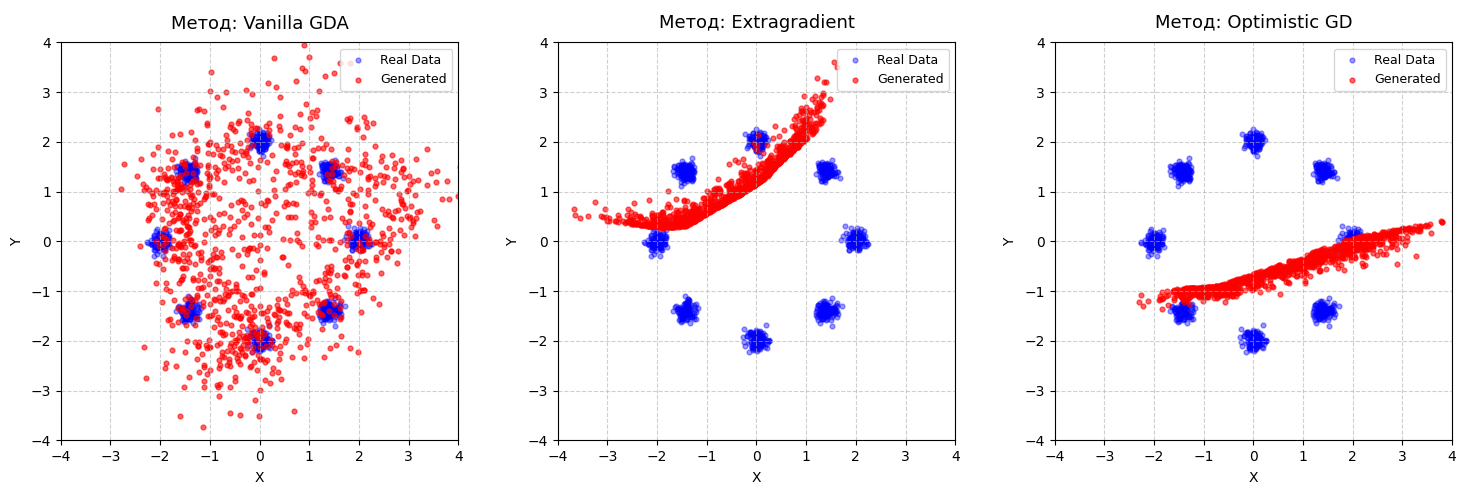
\includegraphics[width=1.0\textwidth]{Figure_2.png} 
			\caption{Траектории параметров $(\theta_G, \theta_D)$ и спектр Якобиана $J$ для методов Vanilla GDA, Extragradient и Optimistic GD в 2D toy-GAN. Метод Vanilla GDA демонстрирует нестабильное поведение: наблюдается чистое вращение параметров, приводящее к разлёту сгенерированных данных и невозможности восстановления структуры мод. Методы Extragradient и Optimistic GD формируют отрицательную симметричную часть в эффективном Якобиане, что приводит к демпфированию ротации, устойчивой динамике и успешной аппроксимации целевого распределения.}
			\label{fig:gan_experiment_results}
	\end{figure}

	
	\subsection{Вывод по разделу}
	Экспериментальное исследование подтверждает, что методы экстраградиентного типа (\textit{Extragradient, OGDA}) обладают наибольшей теоретической и практической эффективностью в подавлении игровой ротации за счет естественного формирования отрицательной симметричной части в эффективном Якобиане системы. 
	
 Базовый метод \textit{Vanilla GDA} без дополнительных модификаций остается строго вращательным и непригодным для поиска устойчивых равновесий Нэша. 
	\section{Абляция и сравнительный анализ}
	
	Для детального изучения свойств алгоритмов был проведен численный абляционный анализ, в ходе которого исследовалось влияние гиперпараметров (размера шага, регуляризации и шума) на сходимость и устойчивость траекторий.
	
	Величина шага обучения $\eta$ является критическим параметром, определяющим баланс между скоростью сходимости и устойчивостью игровой динамики. На основе серии экспериментов были сделаны следующие выводы:
	\begin{itemize}
		\item \textbf{Vanilla GDA:} Метод демонстрирует расходимость при любых фиксированных значениях шага $\eta$. При малых шагах (например, $\eta = 0.001$) траектория медленно раскручивается по спирали наружу, а при увеличении шага ($\eta \ge 0.01$) мгновенно наступает численный взрыв градиентов.
		\item \textbf{Extragradient (EG):} Алгоритм подтверждает теоретически выведенную верхнюю границу устойчивости по шагу ($\eta < 1/\|M\|_2$). При оптимальном шаге наблюдается быстрая и плавная сходимость к центрам всех 8 гауссиан. Однако при чрезмерном завышении шага предикторная точка слишком сильно искажает направление основного шага, что приводит к нарушению монотонности и потере устойчивости.
		\item \textbf{Optimistic GD (OGD):} Метод более чувствителен к выбору шага, чем EG, поскольку аппроксимация экстраполяции использует «устаревший» градиент с предыдущего шага. OGD демонстрирует отличную сходимость при умеренных значениях $\eta$, но при больших шагах история градиентов начинает вносить фазовую задержку, что дестабилизирует систему и возвращает её к циклическим режимам.
	\end{itemize}
	
	Поскольку экстраградиентный метод выполняет два прохода (forward/backward) за одну итерацию, честное сравнение алгоритмов требует сопоставления не по числу формальных шагов, а по реальному вычислительному бюджету (количеству вычислений градиента). 
	
	При одинаковом числе итераций ($N=3000$) метод OGD работает почти в два раза быстрее, чем EG, и при этом обеспечивает сопоставимое качество аппроксимации целевого распределения. Если же ограничить обе схемы одинаковым временем работы (что эквивалентно $N$ итераций для EG и $2N$ итераций для OGD), оптимистичный подход успевает точнее демпфировать колебания высокого порядка, точечно распределяя сгенерированные объекты по модам датасета.
	
	Добавление дополнительных стохастических и детерминированных стабилизаторов оказывает выраженное влияние на геометрию векторного поля:
	\begin{itemize}
		\item \textbf{Слабая регуляризация } Математически добавление штрафа вида $\frac{1}{2}\gamma \|\theta\|^2$ приводит к появлению члена $-\gamma \theta$ в векторном поле. Это эквивалентно добавлению строго положительно определенной матрицы $\gamma I$ в симметричную часть Якобиана $S$. Такая модификация смещает вещественные части собственных значений влево, что стабилизирует даже стандартный GDA, заставляя его траектории затухать к центру. Однако избыточная регуляризация смещает само положение равновесия Нэша, ухудшая финальное качество генерации.
		\item \textbf{Инъекция шума:} Добавление слабого гауссова шума в латентный код или к признакам дискриминатора действует как стохастическая регуляризация. Шум размывает сингулярные области векторного поля и эффективно сглаживает Якобиан, помогая методам EG и OGD не застревать в локальных псевдоравновесиях и обеспечивая более равномерное покрытие всех 8 мод распределения.
	\end{itemize}
	
	\begin{table}[h!]
		\centering
		\caption{Сводные результаты абляционного анализа ($N = 3000$ итераций)}
		\label{tab:ablation}
		\begin{tabular}{lcccc}
			\hline
			\textbf{Метод} & \textbf{Шаг $\eta$} & \textbf{Регуляризация} & \textbf{Шум} & \textbf{Режим сходимости} \\ \hline
			Vanilla GDA   & 0.01   & Нет                    & Нет          & Расходимость / Коллапс мод \\ 
			Vanilla GDA   & 0.01   & $L_2$ ($\gamma=0.005$) & Нет          & Слабая сходимость (размытая) \\ \hline
			Extragradient & 0.001  & Нет                    & Нет          & Медленная сходимость \\ 
			Extragradient & 0.01   & Нет                    & Нет          & \textbf{Четкая сходимость (8 мод)} \\ 
			Extragradient & 0.05   & Нет                    & Нет          & Численный взрыв \\ \hline
			Optimistic GD & 0.01   & Нет                    & Нет          & \textbf{Четкая сходимость (8 мод)} \\ 
			Optimistic GD & 0.01   & Нет                    & Да           & Стабильная сходимость, лучшая гладкость \\ \hline
		\end{tabular}
	\end{table}
	
	\section{Вывод }
	
	В ходе выполнения учебной научно-исследовательской работы была исследована проблема устойчивости обучения генеративно-состязательных сетей с позиции теории вариационных неравенств, монотонных операторов и спектрального анализа локальной игровой динамики.
	
	Был выполнен переход от локального линейного анализа поведения GAN к более общей математической постановке через минимаксные задачи и вариационные неравенства. Показано, что обучение генеративно-состязательной сети естественным образом интерпретируется как задача поиска равновесия Нэша или нуля связанного векторного поля. Это позволяет использовать развитый аппарат теории монотонных операторов для анализа устойчивости и сходимости игровых алгоритмов оптимизации.
	
	На модельном примере билинейной игры строго показано, что стандартный метод градиентного спуска-восхождения ( GDA) не обладает свойством сходимости и порождает расходящиеся вращательные траектории. В противоположность этому экстраградиентный и оптимистичный методы формируют дополнительную стабилизирующую компоненту второго порядка, эквивалентную внесению отрицательно полуопределенной симметричной части в эффективную матрицу динамики, что подавляет игровые осцилляции и обеспечивает устойчивость алгоритма.

	\section{Заключение}
	
	Настоящая работа была посвящена исследованию устойчивости обучения генеративно-состязательных сетей с использованием современных математических методов анализа игровых систем. Основной акцент был сделан на переходе от локального анализа линейной динамики к более общей операторной постановке, основанной на вариационных неравенствах и свойствах монотонности.
	
	Проведенное исследование показывает, что проблемы нестабильности GAN имеют фундаментальную математическую природу и обусловлены преобладанием вращательной компоненты в игровой динамике. Классические методы первого порядка, ориентированные исключительно на локальный градиент, оказываются недостаточными в состязательной среде, поскольку не учитывают структуру взаимодействия между участниками игры.
	
	Использование экстраградиентных и оптимистичных методов демонстрирует, что включение механизма предсказания поведения векторного поля позволяет существенно повысить устойчивость обучения.
	Полученные результаты обладают не только теоретической значимостью, но и практической ценностью для построения более устойчивых алгоритмов генеративного моделирования. Представленный подход к анализу через спектральные свойства Якобиана и операторную монотонность может быть использован для исследования более сложных архитектур.
	\section{Репозиторий и воспроизводимость}
	Полный исходный код  выложен в открытый репозиторий для полной воспроизводимости по адресу: \\
	\url{https://github.com/fansroretet7-afk/gan-stability-convergence-plots}
	
	\section{Список литературы}
	\begin{thebibliography}{99}
		
		\bibitem{goodfellow2014} I. Goodfellow, J. Pouget-Abadie, M. Mirza, B. Xu, D. Warde-Farley, S. Ozair, A. Courville, and Y. Bengio. Generative Adversarial Nets. In \textit{Advances in Neural Information Processing Systems}, 2014.
		
		\bibitem{nagarajan2017} V. Nagarajan and J. Z. Kolter. Gradient Descent GAN Optimization is Locally Stable. In \textit{Advances in Neural Information Processing Systems}, 2017.
		
		\bibitem{mescheder2018} L. Mescheder, A. Geiger, and S. Nowozin. Which Training Methods for GANs do actually Converge? In \textit{Proceedings of the 35th International Conference on Machine Learning}, 2018.
		
		\bibitem{heusel2017} M. Heusel, H. Ramsauer, T. Unterthiner, B. Nessler, and S. Hochreiter. GANs Trained by a Two Time-Scale Update Rule Converge to a Local Nash Equilibrium. In \textit{Advances in Neural Information Processing Systems}, 2017.
		
		\bibitem{daskalakis2018} C. Daskalakis, A. Ilyas, V. Syrgkanis, and H. Zeng. Training GANs with Optimism. In \textit{International Conference on Learning Representations}, 2018.
		
		\bibitem{gidel2019} G. Gidel, H. Berard, G. Vignoud, P. Vincent, and S. Lacoste-Julien. A Variational Inequality Perspective on Generative Adversarial Networks. In \textit{International Conference on Learning Representations}, 2019.
		
		\bibitem{korpelevich1976} Г. М. Корпелевич. Экстраградиентный метод для нахождения седловых точек и других задач. \textit{Экономика и математические методы}, 12(4):747--756, 1976.
		
		\bibitem{nemirovski2004} A. Nemirovski. Prox-Method with Rate of Convergence O(1/t) for Variational Inequalities with Lipschitz Continuous Monotone Operators and Smooth Convex-Concave Saddle Point Problems. \textit{SIAM Journal on Optimization}, 15(1):229--251, 2004.
		
		\bibitem{popov1980} L. D. Popov. A Modification of the Arrow--Hurwicz Method for Search of Saddle Points. \textit{Mathematical Notes of the Academy of Sciences of the USSR}, 28(5):845--848, 1980.
		
		\bibitem{goodfellow2016} I. Goodfellow, Y. Bengio, and A. Courville. \textit{Deep Learning}. MIT Press, 2016.
		
		\bibitem{nikolenko2018} С. Николенко, А. Кадурин, Е. Архангельская. \textit{Глубокое обучение. Погружение в мир нейронных сетей}. Санкт-Петербург: Питер, 2018.
		
	\end{thebibliography}
	
\end{document}
